\documentclass[10pt]{article}
\usepackage[margin=1in]{geometry}
\usepackage[utf8]{inputenc}
\usepackage[english]{babel}
\usepackage[T1]{fontenc}
\usepackage{fourier}
\usepackage{amsthm}
\usepackage{amssymb}
\usepackage{amsmath}
\usepackage{amsfonts}
\usepackage{latexsym}
\usepackage{graphicx}
\usepackage{float}
\usepackage{etoolbox}
\usepackage{hyperref}
\usepackage{tikz}
\usepackage{lipsum}


\newcommand{\R}{\mathbb{R}}
\newcommand{\N}{\mathbb{N}}
\newcommand{\Z}{\mathbb{Z}}
\newcommand{\Q}{\mathbb{Q}}
\newcommand{\C}{\mathbb{C}}


\title{Assignment I: The softmax function}
\author{Luca Lombardo}
\date{}

\begin{document}
\maketitle

\tableofcontents

\setlength{\parindent}{0em}
% \setlength{\parskip}{1em}

% \section{Introduction}
% The softmax function is a mathematical function that takes a vector of real numbers as input and transforms it into a probability distribution. The mathematical definition of the softmax function is given by:

% \begin{equation*}
%     \sigma: \R^K \to \Big\{ z \in \R^K \,|\, z_i \geq 0, \sum_{i=1}^K z_i = 1 \Big\}
% \end{equation*}
% \begin{equation}
%     \sigma(\mathbf{z}_j) = \frac{e^{z_j}}{\sum_{i=1}^K e^{z_i}}
% \end{equation}

\section{Implementations}
In the following sections, given a scalar implementation (to witch we will refer as \texttt{softmax\_plain}), we will show how to auto-vectorize it and then how to manually vectorize the code using AVX intrinsics and FMA. Then we will compare the results of the three implementations.

\subsection{Auto-Vectorized implementation}
The auto-vectorized version of the softmax function includes several optimizations. \texttt{\#pragma omp simd} directives were added to vectorize the main computational loops, with reduction clauses for correct maximum value and sum calculations. The \texttt{expf()} function replaced \texttt{std::exp()} for better SIMD performance. Precomputing the inverse sum (\texttt{inv\_sum = 1.0f / sum}) and using multiplications instead of divisions improved efficiency. Explicit comparisons replaced \texttt{std::max()} to aid vectorization. Using \texttt{\#pragma omp parallel for simd} degraded performance for small arrays due to thread management overhead but scaled well for large arrays.

\subsection{Manually Vectorized implementation}
The \texttt{softmax\_avx} implementation employs a three-phase approach with explicit AVX2 intrinsics to achieve maximum performance. Each phase (find maximum, compute exponentials with sum, normalize) is optimized with loop unrolling (4x for processing 32 elements at once), software prefetching, and efficient horizontal reduction patterns. To handle array sizes that aren't multiples of 8 (AVX register width), a principled masking approach is used via the \texttt{compute\_mask()} function, which creates appropriate mask vectors for conditional loading/storing operations (\texttt{\_mm256\_maskload\_ps} and \texttt{\_mm256\_maskstore\_ps}). This eliminates the need for a remainder loop, improving instruction throughput. The implementation also employs careful cache blocking with a 32KB block size to minimize L1 cache misses during multi-phase processing, crucial since the algorithm makes multiple passes over the data. \\

The implementation utilizes OpenMP to distribute computation across available hardware threads. For the reduction phase (finding the maximum), a standard \texttt{\#pragma omp parallel for reduction(max:max\_val)} is used, while the sum calculation employs a more specific approach with manual local reductions and atomic updates to minimize false sharing and synchronization overhead. Performance analysis revealed that small array sizes suffered from OpenMP thread management overhead, leading to a specialized variant that skips parallelization entirely for small inputs while maintaining all AVX optimizations.

\section{Results}
In this section, we compare the three implementations of the softmax function under different conditions. First, we evaluate the \texttt{softmax\_auto} implementation with and without the \texttt{parallel} directive. Next, we compare the performance using AVX2 and AVX512 instructions. The \texttt{softmax\_auto} relies on the compiler's auto-vectorization, which benefits from AVX512 if available. We expect \texttt{softmax\_auto} with AVX512 to outperform \texttt{softmax\_avx}, which is manually optimized for AVX2. Without AVX512 support, \texttt{softmax\_avx} should have better performance.

\paragraph{How do we measure the performance?}
Performance is measured using a rigorous benchmark: after 3 warmup iterations, 11 samples (each averaging 20 iterations) are taken and the median is reported. Input sizes vary from 1 to 1,048,576 elements (both powers of 2 and non-power-of-2) to test alignment. A custom C++17 aligned allocator (32-byte alignment) ensures fair SIMD comparisons. Correctness is verified by checking that each implementation produces equivalent probability distributions (non-negative values summing to 1), and speedups are reported relative to the plain implementation.

\paragraph{Numerical stability} The softmax function can be numerically unstable, especially for large values. To ensure stability during benchmarks, input values are limited to $1048576$.

\subsection{Benchmarks}
\paragraph{No AVX512} The results, depicted in Figure \ref{fig:softmax_auto_no_avx512}, illustrate the performance without the \texttt{parallel} directive in the \texttt{softmax\_auto} implementation. This pattern is consistent even for smaller input sizes. On the other hand, enabling the \texttt{parallel} directive significantly enhances the performance of \texttt{softmax\_auto} for large input sizes, as illustrated in Figure \ref{fig:softmax_auto_no_avx512_parallel}. The performance approaches that of \texttt{softmax\_avx}. However, for small input sizes, the overhead introduced by the \texttt{parallel} directive outweighs the benefits of parallelization, resulting in a performance degradation compared to the plain implementation.

\begin{figure}[h!]
  \centering
  \begin{minipage}{0.49\textwidth}
    \centering
    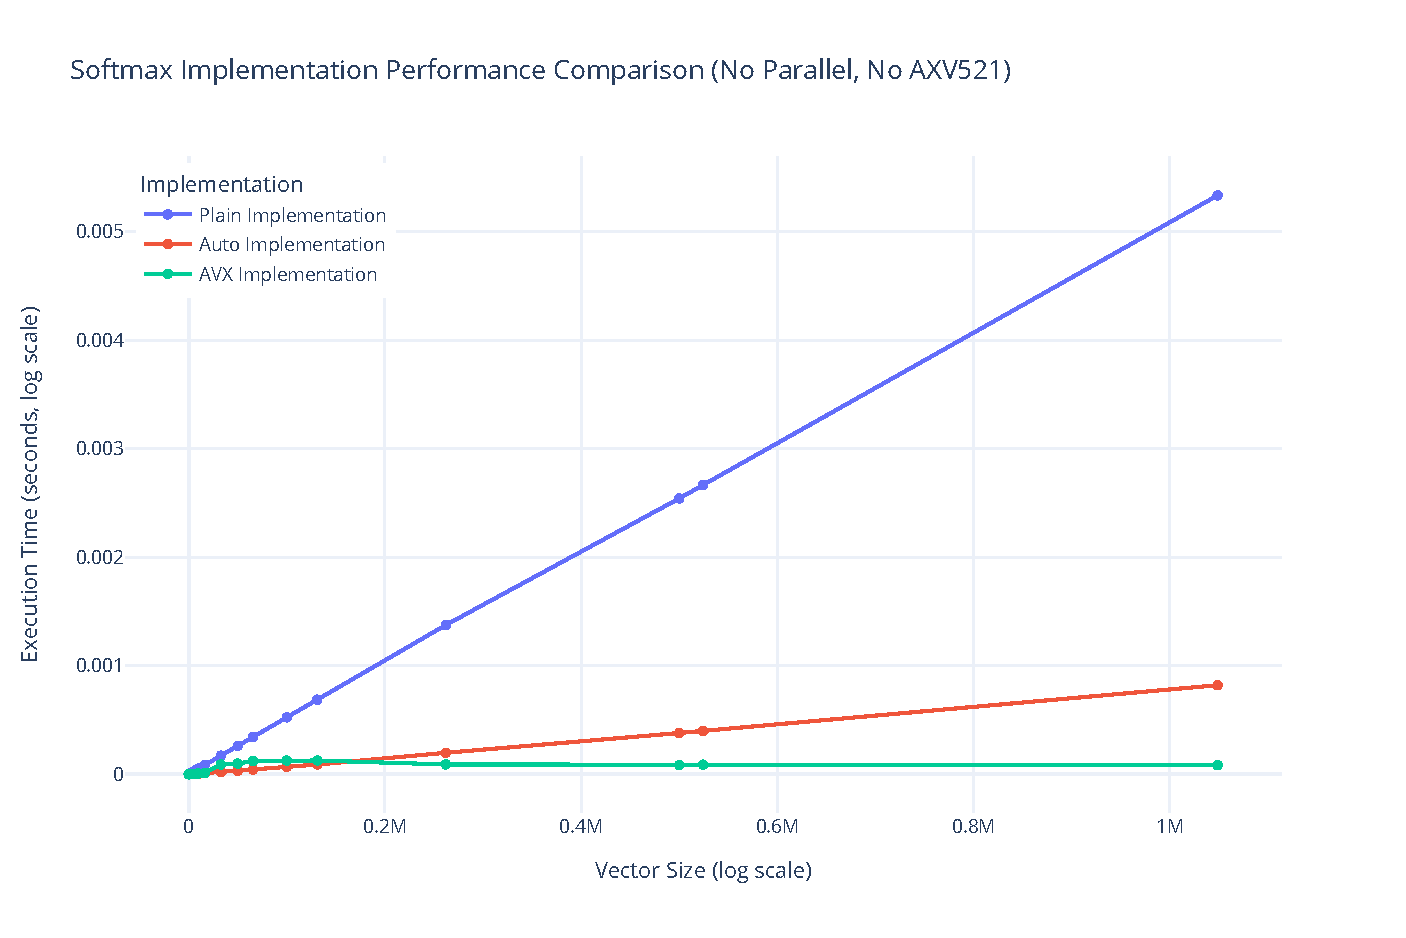
\includegraphics[width=\linewidth]{../images/softmax_noparallel_noaxv521.pdf}
    \caption{Performance comparison without AVX512 support and without the \texttt{parallel} directive.}
    \label{fig:softmax_auto_no_avx512}
  \end{minipage}%
  \hfill
  \begin{minipage}{0.49\textwidth}
    \centering
    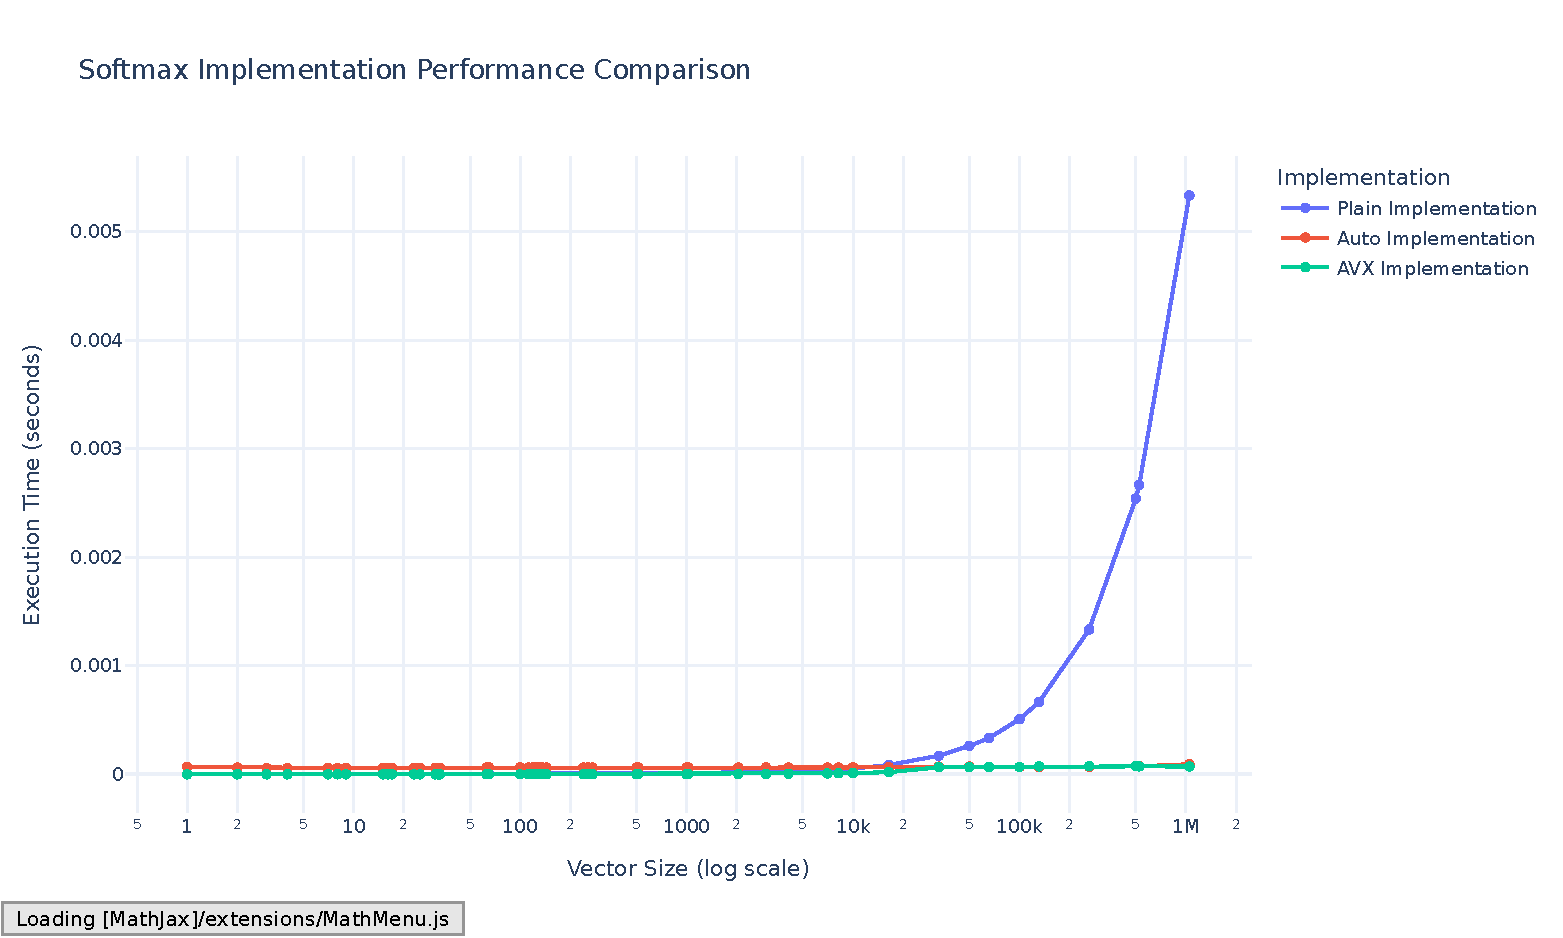
\includegraphics[width=\linewidth]{../images/softmax_parallel_noaxv521.pdf}
    \caption{Performance comparison without AVX512 support and with the \texttt{parallel} directive.}
    \label{fig:softmax_auto_no_avx512_parallel}
  \end{minipage}
\end{figure}

\paragraph{With AVX512} When compiled with AVX512 support, the \texttt{softmax\_auto} implementation demonstrates similar performance to the \texttt{softmax\_avx} implementation for small input sizes without the \texttt{parallel} directive. However, for larger input sizes, \texttt{softmax\_avx} performs better (See Figure \ref{fig:softmax_auto_avx512_no_parallel}). Enabling the \texttt{parallel} directive allows \texttt{softmax\_auto} to surpass \texttt{softmax\_avx} in performance for large input sizes, though the overhead for small input sizes remains a limiting factor (See Figure \ref{fig:softmax_auto_avx512_parallel}).

\clearpage
\begin{figure}[ht!]
  \centering
  \begin{minipage}{0.49\textwidth}
    \centering
    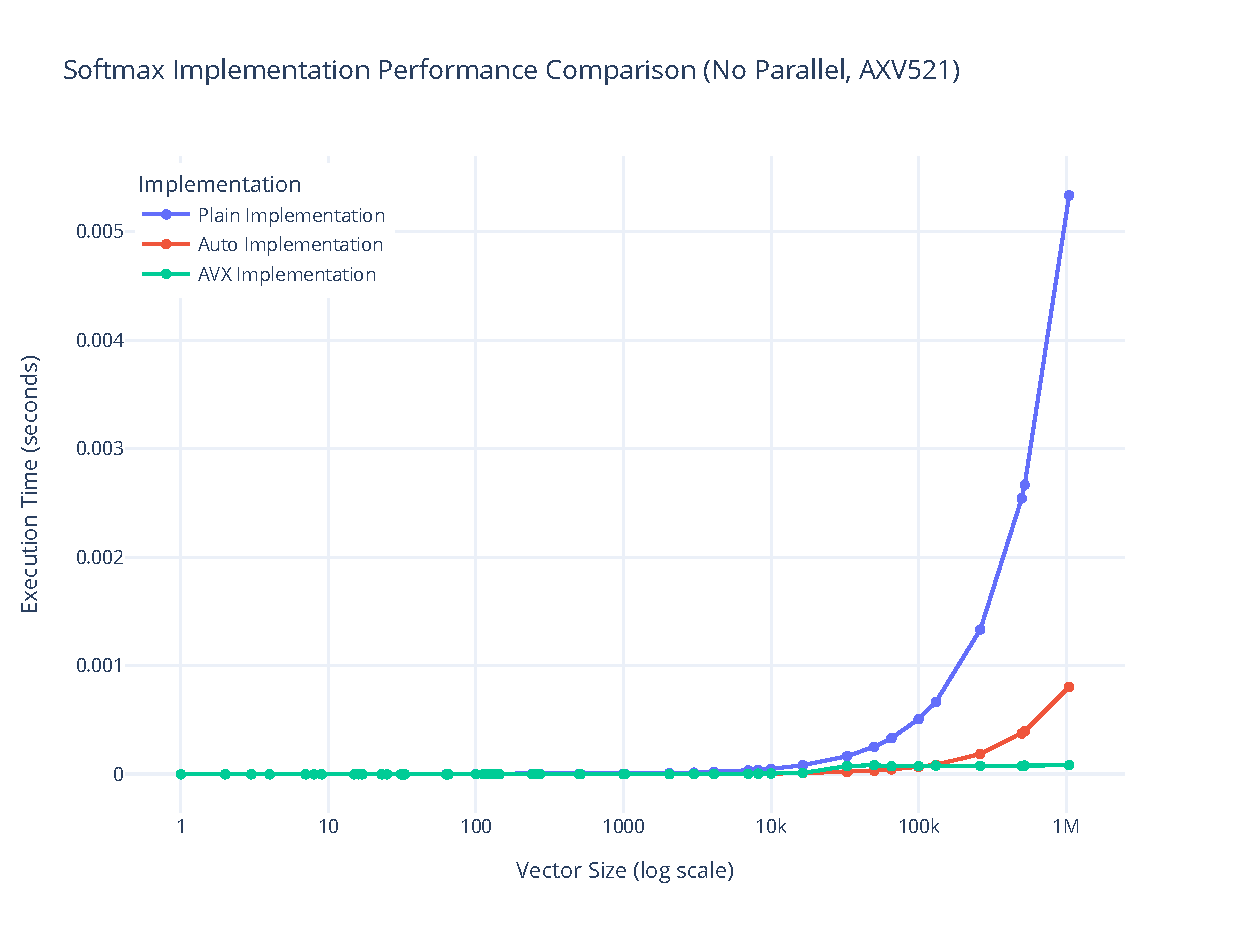
\includegraphics[width=\linewidth]{../images/softmax_noparallel_axv521.pdf}
    \caption{Performance comparison with AVX512 support and without the \texttt{parallel} directive.}
    \label{fig:softmax_auto_avx512_no_parallel}
  \end{minipage}%
  \hfill
  \begin{minipage}{0.49\textwidth}
    \centering
    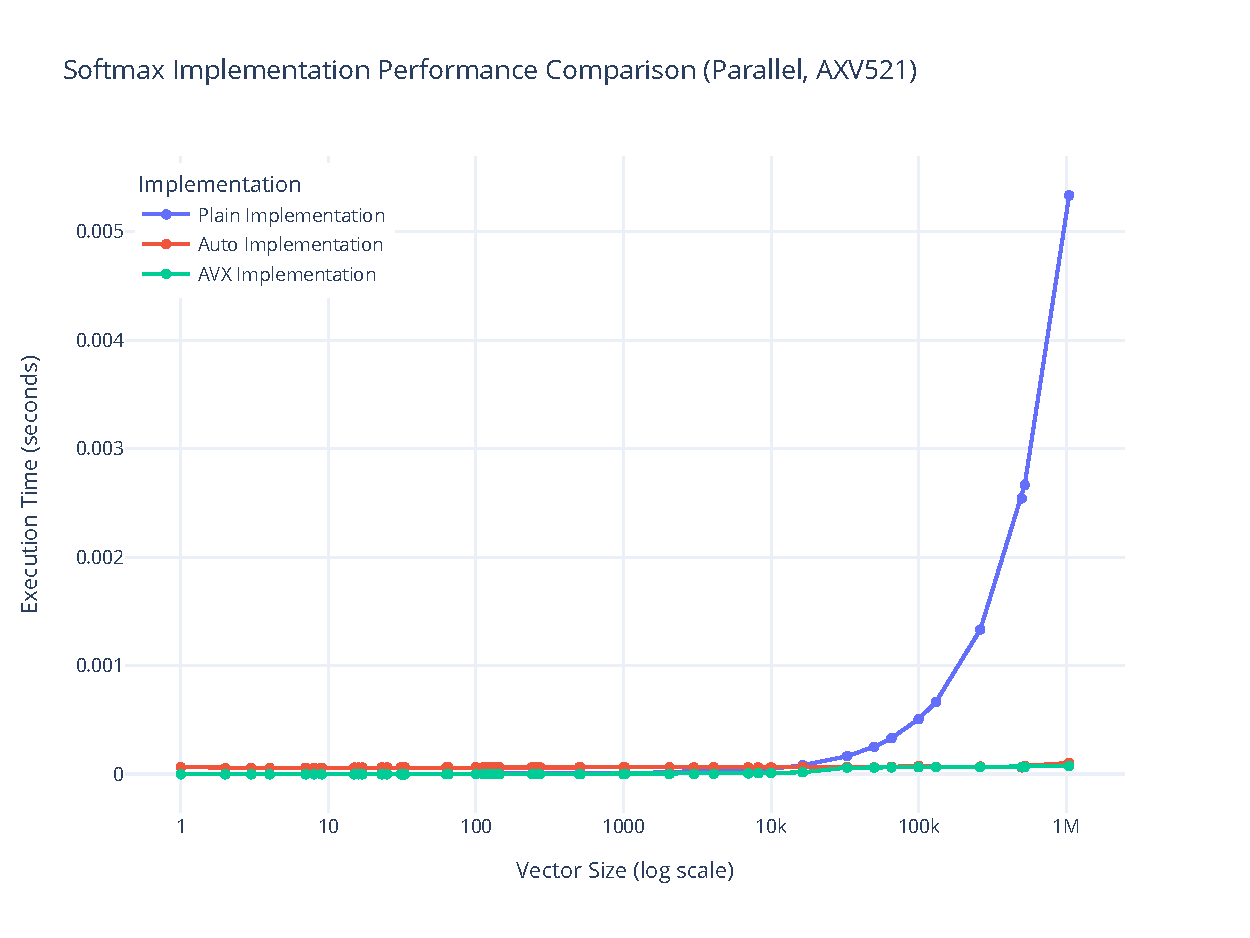
\includegraphics[width=\linewidth]{../images/softmax_parallel_axv521.pdf}
    \caption{Performance comparison with AVX512 support and with the \texttt{parallel} directive.}
    \label{fig:softmax_auto_avx512_parallel}
  \end{minipage}
\end{figure}

In addition to performance, we also analyze the speedup of the \texttt{softmax\_auto} implementation relative to the plain implementation with AVX512 support and without the \texttt{parallel} directive. The results are shown in Figures \ref{fig:softmax_auto_avx512_no_parallel_speedup} and \ref{fig:softmax_auto_avx512_parallel_speedup}. The speedup is significant for large input sizes, especially when using the \texttt{parallel} directive.

\begin{figure}[h!]
  \centering
  \begin{minipage}{0.49\textwidth}
    \centering
    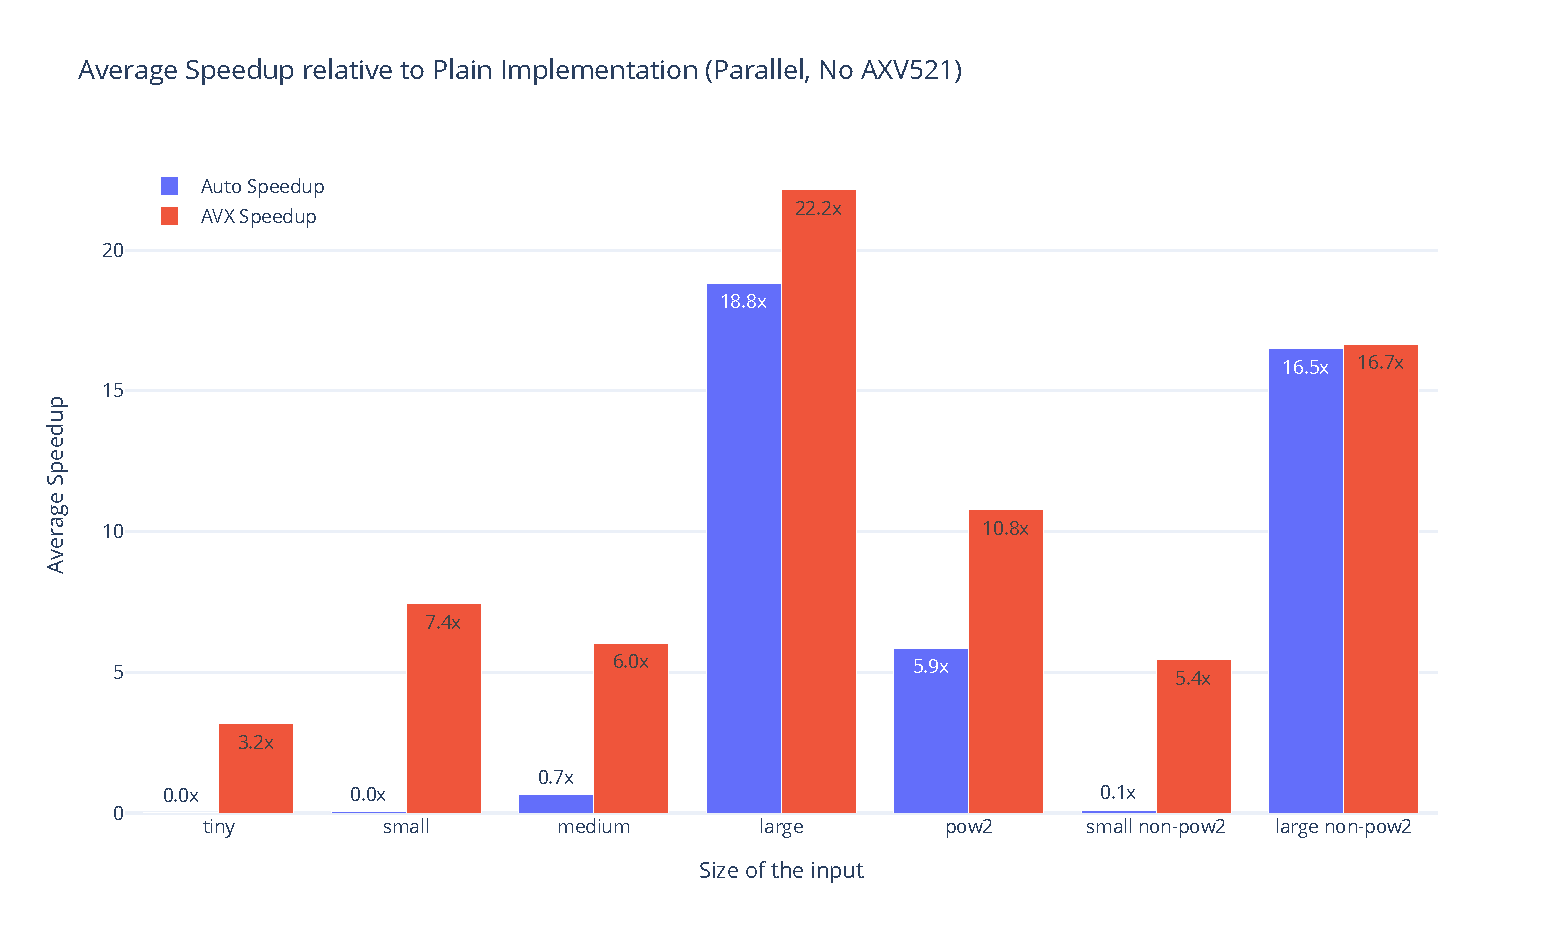
\includegraphics[width=\linewidth]{../images/softmax_parallel_axv521_speedup.pdf}
    \caption{Speedup with AVX512 support and with the \texttt{parallel} directive.}
    \label{fig:softmax_auto_avx512_no_parallel_speedup}
  \end{minipage}%
  \hfill
  \begin{minipage}{0.49\textwidth}
    \centering
    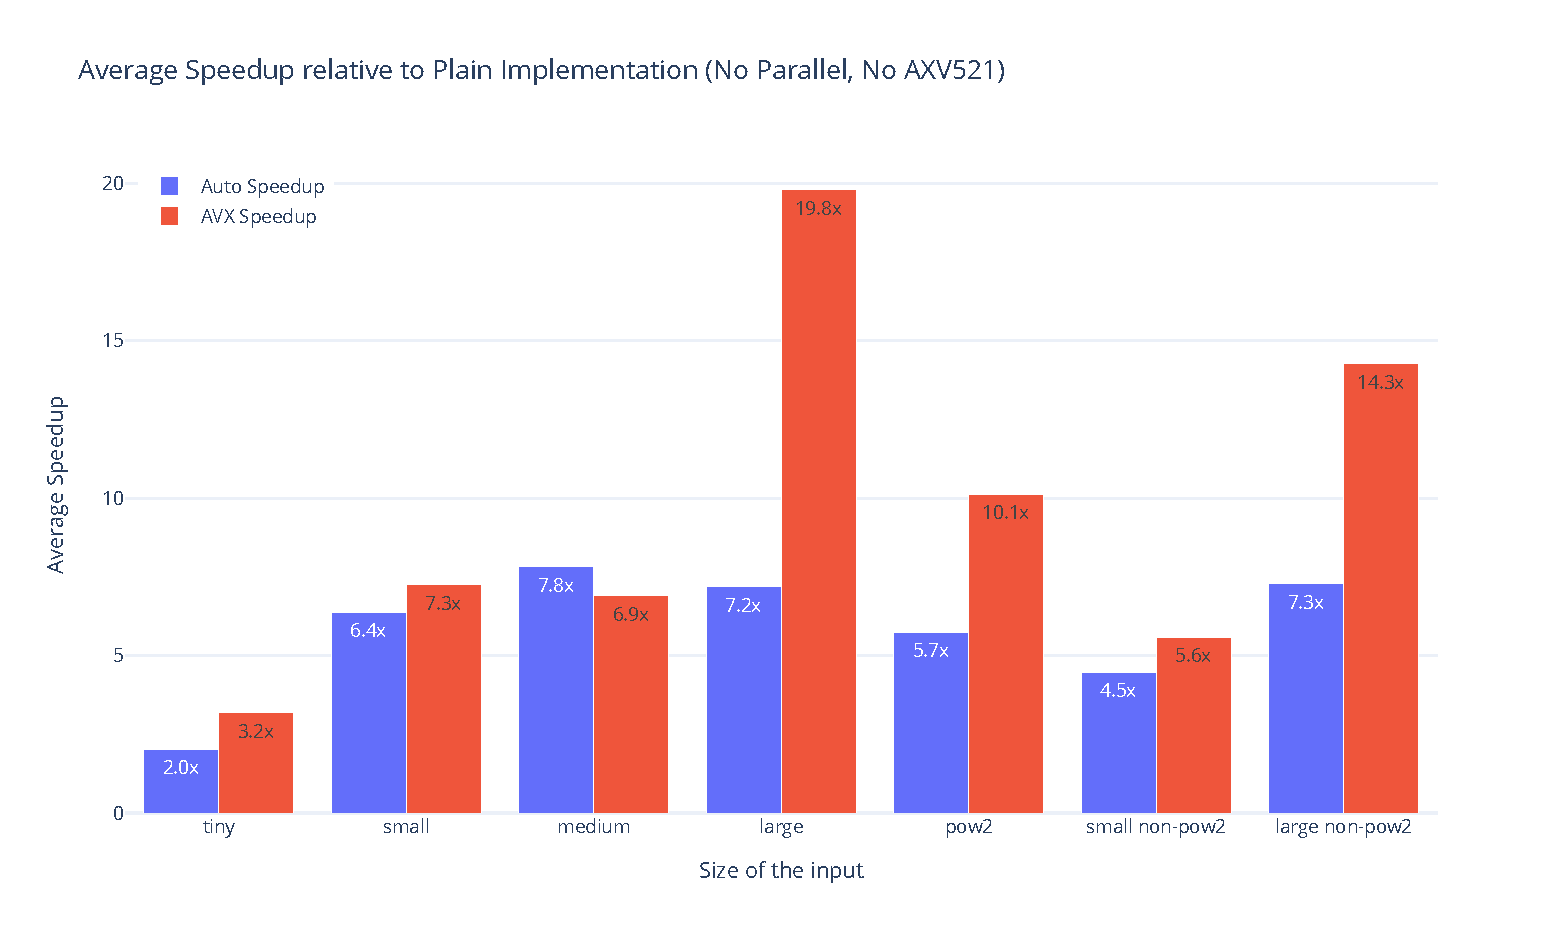
\includegraphics[width=\linewidth]{../images/softmax_noparallel_axv521_speedup.pdf}
    \caption{Speedup with AVX512 support and without the \texttt{parallel} directive.}
    \label{fig:softmax_auto_avx512_parallel_speedup}
  \end{minipage}
\end{figure}

\subsection{Compilation and Execution}
The implementation uses different compilation flags to optimize for different instruction sets and vectorization capabilities. The \texttt{OPTFLAGS} variable enables level 3 optimizations (\texttt{-O3}), fast math operations (\texttt{-ffast-math}), and OpenMP support. For the auto-vectorized implementation, \texttt{AUTOFLAGS} includes \texttt{-mavx2} to enable AVX2 instructions and \texttt{-ftree-vectorize} to explicitly request vectorization. During testing, we compiled with both \texttt{-mavx2} and \texttt{-march=native} settings to evaluate performance with AVX2 and AVX512 instructions respectively. The manually vectorized implementation uses \texttt{AVXFLAGS} with \texttt{-mavx2}, \texttt{-mfma} to enable fused multiply-add operations, and alignment optimizations (\texttt{-malign-double} and \texttt{-falign-loops=32}). To build all implementations, run \texttt{make all} in the project directory. The command \texttt{make test} builds and executes the test suite that verifies correctness across all implementations and saves the results to a .csv file. Individual executables can be built using \texttt{make softmax\_plain}, \texttt{make softmax\_auto}, or \texttt{make softmax\_avx}.



\end{document}
